\documentclass[]{book}
\usepackage{lmodern}
\usepackage{amssymb,amsmath}
\usepackage{ifxetex,ifluatex}
\usepackage{fixltx2e} % provides \textsubscript
\ifnum 0\ifxetex 1\fi\ifluatex 1\fi=0 % if pdftex
  \usepackage[T1]{fontenc}
  \usepackage[utf8]{inputenc}
\else % if luatex or xelatex
  \ifxetex
    \usepackage{mathspec}
  \else
    \usepackage{fontspec}
  \fi
  \defaultfontfeatures{Ligatures=TeX,Scale=MatchLowercase}
\fi
% use upquote if available, for straight quotes in verbatim environments
\IfFileExists{upquote.sty}{\usepackage{upquote}}{}
% use microtype if available
\IfFileExists{microtype.sty}{%
\usepackage{microtype}
\UseMicrotypeSet[protrusion]{basicmath} % disable protrusion for tt fonts
}{}
\usepackage{hyperref}
\hypersetup{unicode=true,
            pdftitle={Predictive-Analytics-MAS-R-Study-Manual},
            pdfauthor={Sam Castillo; Brian Fannin},
            pdfborder={0 0 0},
            breaklinks=true}
\urlstyle{same}  % don't use monospace font for urls
\usepackage{natbib}
\bibliographystyle{apalike}
\usepackage{color}
\usepackage{fancyvrb}
\newcommand{\VerbBar}{|}
\newcommand{\VERB}{\Verb[commandchars=\\\{\}]}
\DefineVerbatimEnvironment{Highlighting}{Verbatim}{commandchars=\\\{\}}
% Add ',fontsize=\small' for more characters per line
\usepackage{framed}
\definecolor{shadecolor}{RGB}{248,248,248}
\newenvironment{Shaded}{\begin{snugshade}}{\end{snugshade}}
\newcommand{\AlertTok}[1]{\textcolor[rgb]{0.94,0.16,0.16}{#1}}
\newcommand{\AnnotationTok}[1]{\textcolor[rgb]{0.56,0.35,0.01}{\textbf{\textit{#1}}}}
\newcommand{\AttributeTok}[1]{\textcolor[rgb]{0.77,0.63,0.00}{#1}}
\newcommand{\BaseNTok}[1]{\textcolor[rgb]{0.00,0.00,0.81}{#1}}
\newcommand{\BuiltInTok}[1]{#1}
\newcommand{\CharTok}[1]{\textcolor[rgb]{0.31,0.60,0.02}{#1}}
\newcommand{\CommentTok}[1]{\textcolor[rgb]{0.56,0.35,0.01}{\textit{#1}}}
\newcommand{\CommentVarTok}[1]{\textcolor[rgb]{0.56,0.35,0.01}{\textbf{\textit{#1}}}}
\newcommand{\ConstantTok}[1]{\textcolor[rgb]{0.00,0.00,0.00}{#1}}
\newcommand{\ControlFlowTok}[1]{\textcolor[rgb]{0.13,0.29,0.53}{\textbf{#1}}}
\newcommand{\DataTypeTok}[1]{\textcolor[rgb]{0.13,0.29,0.53}{#1}}
\newcommand{\DecValTok}[1]{\textcolor[rgb]{0.00,0.00,0.81}{#1}}
\newcommand{\DocumentationTok}[1]{\textcolor[rgb]{0.56,0.35,0.01}{\textbf{\textit{#1}}}}
\newcommand{\ErrorTok}[1]{\textcolor[rgb]{0.64,0.00,0.00}{\textbf{#1}}}
\newcommand{\ExtensionTok}[1]{#1}
\newcommand{\FloatTok}[1]{\textcolor[rgb]{0.00,0.00,0.81}{#1}}
\newcommand{\FunctionTok}[1]{\textcolor[rgb]{0.00,0.00,0.00}{#1}}
\newcommand{\ImportTok}[1]{#1}
\newcommand{\InformationTok}[1]{\textcolor[rgb]{0.56,0.35,0.01}{\textbf{\textit{#1}}}}
\newcommand{\KeywordTok}[1]{\textcolor[rgb]{0.13,0.29,0.53}{\textbf{#1}}}
\newcommand{\NormalTok}[1]{#1}
\newcommand{\OperatorTok}[1]{\textcolor[rgb]{0.81,0.36,0.00}{\textbf{#1}}}
\newcommand{\OtherTok}[1]{\textcolor[rgb]{0.56,0.35,0.01}{#1}}
\newcommand{\PreprocessorTok}[1]{\textcolor[rgb]{0.56,0.35,0.01}{\textit{#1}}}
\newcommand{\RegionMarkerTok}[1]{#1}
\newcommand{\SpecialCharTok}[1]{\textcolor[rgb]{0.00,0.00,0.00}{#1}}
\newcommand{\SpecialStringTok}[1]{\textcolor[rgb]{0.31,0.60,0.02}{#1}}
\newcommand{\StringTok}[1]{\textcolor[rgb]{0.31,0.60,0.02}{#1}}
\newcommand{\VariableTok}[1]{\textcolor[rgb]{0.00,0.00,0.00}{#1}}
\newcommand{\VerbatimStringTok}[1]{\textcolor[rgb]{0.31,0.60,0.02}{#1}}
\newcommand{\WarningTok}[1]{\textcolor[rgb]{0.56,0.35,0.01}{\textbf{\textit{#1}}}}
\usepackage{longtable,booktabs}
\usepackage{graphicx,grffile}
\makeatletter
\def\maxwidth{\ifdim\Gin@nat@width>\linewidth\linewidth\else\Gin@nat@width\fi}
\def\maxheight{\ifdim\Gin@nat@height>\textheight\textheight\else\Gin@nat@height\fi}
\makeatother
% Scale images if necessary, so that they will not overflow the page
% margins by default, and it is still possible to overwrite the defaults
% using explicit options in \includegraphics[width, height, ...]{}
\setkeys{Gin}{width=\maxwidth,height=\maxheight,keepaspectratio}
\IfFileExists{parskip.sty}{%
\usepackage{parskip}
}{% else
\setlength{\parindent}{0pt}
\setlength{\parskip}{6pt plus 2pt minus 1pt}
}
\setlength{\emergencystretch}{3em}  % prevent overfull lines
\providecommand{\tightlist}{%
  \setlength{\itemsep}{0pt}\setlength{\parskip}{0pt}}
\setcounter{secnumdepth}{5}
% Redefines (sub)paragraphs to behave more like sections
\ifx\paragraph\undefined\else
\let\oldparagraph\paragraph
\renewcommand{\paragraph}[1]{\oldparagraph{#1}\mbox{}}
\fi
\ifx\subparagraph\undefined\else
\let\oldsubparagraph\subparagraph
\renewcommand{\subparagraph}[1]{\oldsubparagraph{#1}\mbox{}}
\fi

%%% Use protect on footnotes to avoid problems with footnotes in titles
\let\rmarkdownfootnote\footnote%
\def\footnote{\protect\rmarkdownfootnote}

%%% Change title format to be more compact
\usepackage{titling}

% Create subtitle command for use in maketitle
\providecommand{\subtitle}[1]{
  \posttitle{
    \begin{center}\large#1\end{center}
    }
}

\setlength{\droptitle}{-2em}

  \title{Predictive-Analytics-MAS-R-Study-Manual}
    \pretitle{\vspace{\droptitle}\centering\huge}
  \posttitle{\par}
    \author{Sam Castillo \\ Brian Fannin}
    \preauthor{\centering\large\emph}
  \postauthor{\par}
      \predate{\centering\large\emph}
  \postdate{\par}
    \date{2019-10-14}

\usepackage{booktabs}
\usepackage{amsthm}
\makeatletter
\def\thm@space@setup{%
  \thm@preskip=8pt plus 2pt minus 4pt
  \thm@postskip=\thm@preskip
}
\makeatother

\begin{document}
\maketitle

{
\setcounter{tocdepth}{1}
\tableofcontents
}
\hypertarget{who-is-this-book-for}{%
\chapter{Who is this book for}\label{who-is-this-book-for}}

This book will help you to pass the SOA's Predictive Analytics Exam and give you insights and useful code snippets that will translate into your every day work flow. Additionally, material is also covered which is on the CAS exams MAS-I and MAS-II.

\hypertarget{how-to-use-this-book}{%
\chapter{How to Use this book}\label{how-to-use-this-book}}

This is like any of the other actuarial exam that you have taken. The format is a 5-hr and 15 minute project that uses RStudio, Excel, and Word. There are three essential skills needed to pass. These are

\begin{enumerate}
\def\labelenumi{\arabic{enumi}.}
\tightlist
\item
  R competency;
\item
  Business writing ability;
\item
  Statistics, predictive analytics, and machine learning knowledge.
\end{enumerate}

If you already have some of these skills, then a good strategy is to focus on your weak areas. If you are relatively new to all three, great! This means that you will be able to learn a lot of useful skills by reading this manual.

\hypertarget{about-the-authors}{%
\chapter{About the authors}\label{about-the-authors}}

\textbf{Sam Castillo} has 4+ years of R programming experience while working as an actuarial predictive modeler for the past 3 years. He passed the predictive analytics exam in June of 2019.

\textbf{Brian Fannin} etc, etc

\hypertarget{intro}{%
\chapter{Getting Started}\label{intro}}

\hypertarget{installing-r-and-rstudio}{%
\section{Installing R and Rstudio}\label{installing-r-and-rstudio}}

\begin{enumerate}
\def\labelenumi{\arabic{enumi}.}
\tightlist
\item
  Download R
\item
  Download RStudio
\end{enumerate}

\hypertarget{setting-up}{%
\section{Setting Up}\label{setting-up}}

\hypertarget{using-the-r-version-of-packages-from-the-soa-include-helper-script}{%
\subsection{Using the R version of packages from the SOA (include helper script)}\label{using-the-r-version-of-packages-from-the-soa-include-helper-script}}

You want to use the exact same code that will be on the Prometric Computers. An R library is a software package that provides added flexibility. R is open-source, which means that it is maintained by a community of developers on a volunteer basis.

To change the library that R uses, use the \texttt{libPaths} function.

\begin{Shaded}
\begin{Highlighting}[]
\CommentTok{#.libPaths("C:/Users/sam.castillo/Desktop/PA/library/PAlibrary")}
\end{Highlighting}
\end{Shaded}

\hypertarget{setting-the-r-version}{%
\subsection{Setting the R Version}\label{setting-the-r-version}}

This book uses Rv3.5. To switch between R versions,

Tools -\textgreater{} Global Options -\textgreater{} R Version -\textgreater{} Restart Rstudio

\hypertarget{r-basic-syntax}{%
\section{R basic syntax}\label{r-basic-syntax}}

There are already hundreds of great tutorials online. This will only be a minimal version.

\hypertarget{data-types}{%
\section{Data Types}\label{data-types}}

Each object in R has a different type.

\begin{itemize}
\tightlist
\item
  numeric
\item
  character
\item
  factors
\item
  booleans
\end{itemize}

As well as classes

\begin{itemize}
\tightlist
\item
  matrix
\item
  data frame
\item
  tibble (just another name for a data frame)
\item
  list (most important)
\end{itemize}

\hypertarget{objects}{%
\subsection{Objects}\label{objects}}

\hypertarget{functions}{%
\subsection{Functions}\label{functions}}

\hypertarget{just-copy-someone-eleses-tutorials}{%
\subsection{Just Copy Someone Elese's Tutorials}\label{just-copy-someone-eleses-tutorials}}

\hypertarget{rmd-file-overview}{%
\section{Rmd file overview}\label{rmd-file-overview}}

\hypertarget{read-in-a-data-file-from-local-computer-in-csv-format}{%
\section{Read in a data file from local computer in csv format}\label{read-in-a-data-file-from-local-computer-in-csv-format}}

\hypertarget{data-manipulation}{%
\chapter{Data Manipulation}\label{data-manipulation}}

About two hours in this exam will be spent just on data manipulation. A common complaint from exam takers who are new to R programming is that this takes too long. Putting in extra practice in this area is garanteed to give you a better score because it will free up time that you can use elsewhere.

Each time that you want to ``do something'' to the data, most of the time there is a function that will do this.

\hypertarget{look-at-the-data}{%
\subsection{Look at the data}\label{look-at-the-data}}

The \texttt{head()} or \texttt{glimpse()} functions both suffice.

\begin{Shaded}
\begin{Highlighting}[]
\KeywordTok{library}\NormalTok{(tidyverse)}
\NormalTok{iris }\OperatorTok\StringTok{ }\KeywordTok{head}\NormalTok{()}
\end{Highlighting}
\end{Shaded}

\begin{verbatim}
##   Sepal.Length Sepal.Width Petal.Length Petal.Width Species
## 1          5.1         3.5          1.4         0.2  setosa
## 2          4.9         3.0          1.4         0.2  setosa
## 3          4.7         3.2          1.3         0.2  setosa
## 4          4.6         3.1          1.5         0.2  setosa
## 5          5.0         3.6          1.4         0.2  setosa
## 6          5.4         3.9          1.7         0.4  setosa
\end{verbatim}

\begin{Shaded}
\begin{Highlighting}[]
\NormalTok{iris }\OperatorTok\StringTok{ }\KeywordTok{glimpse}\NormalTok{()}
\end{Highlighting}
\end{Shaded}

\begin{verbatim}
## Observations: 150
## Variables: 5
## $ Sepal.Length <dbl> 5.1, 4.9, 4.7, 4.6, 5.0, 5.4, 4.6, 5.0, 4.4, 4.9,...
## $ Sepal.Width  <dbl> 3.5, 3.0, 3.2, 3.1, 3.6, 3.9, 3.4, 3.4, 2.9, 3.1,...
## $ Petal.Length <dbl> 1.4, 1.4, 1.3, 1.5, 1.4, 1.7, 1.4, 1.5, 1.4, 1.5,...
## $ Petal.Width  <dbl> 0.2, 0.2, 0.2, 0.2, 0.2, 0.4, 0.3, 0.2, 0.2, 0.1,...
## $ Species      <fct> setosa, setosa, setosa, setosa, setosa, setosa, s...
\end{verbatim}

\hypertarget{look-at-summary-statistics}{%
\subsection{Look at summary statistics}\label{look-at-summary-statistics}}

The \texttt{summary()} function is best.

\begin{Shaded}
\begin{Highlighting}[]
\NormalTok{iris }\OperatorTok\StringTok{ }\KeywordTok{summary}\NormalTok{()}
\end{Highlighting}
\end{Shaded}

\begin{verbatim}
##   Sepal.Length    Sepal.Width     Petal.Length    Petal.Width   
##  Min.   :4.300   Min.   :2.000   Min.   :1.000   Min.   :0.100  
##  1st Qu.:5.100   1st Qu.:2.800   1st Qu.:1.600   1st Qu.:0.300  
##  Median :5.800   Median :3.000   Median :4.350   Median :1.300  
##  Mean   :5.843   Mean   :3.057   Mean   :3.758   Mean   :1.199  
##  3rd Qu.:6.400   3rd Qu.:3.300   3rd Qu.:5.100   3rd Qu.:1.800  
##  Max.   :7.900   Max.   :4.400   Max.   :6.900   Max.   :2.500  
##        Species  
##  setosa    :50  
##  versicolor:50  
##  virginica :50  
##                 
##                 
## 
\end{verbatim}

\hypertarget{find-the-dimensions-of-the-data}{%
\subsection{Find the dimensions of the data}\label{find-the-dimensions-of-the-data}}

\begin{Shaded}
\begin{Highlighting}[]
\NormalTok{iris }\OperatorTok\StringTok{ }\KeywordTok{dim}\NormalTok{()}
\end{Highlighting}
\end{Shaded}

\begin{verbatim}
## [1] 150   5
\end{verbatim}

\hypertarget{queries}{%
\subsection{Queries}\label{queries}}

Queries are very similar to SQL. They begin with a ``SELECT'', use ``GROUP BY'' to aggregate, and have a ``WHERE'' to remove records. Unlike SQL, the ordering of these does not matter. ``SELECT'' can come after a ``WHERE''.

dplyr to SQL translation**

\begin{verbatim}
select() -> SELECT
mutate() -> user-defined columns
summarize() -> aggregated columns
left_join() -> LEFT JOIN
filter() -> WHERE
group_by() -> GROUP BY
filter() -> HAVING
arrange() -> ORDER BY
\end{verbatim}

\begin{Shaded}
\begin{Highlighting}[]
\NormalTok{iris }\OperatorTok\StringTok{ }\KeywordTok{select}\NormalTok{(Sepal.Length, Sepal.Width) }\OperatorTok\StringTok{ }\KeywordTok{head}\NormalTok{()}
\end{Highlighting}
\end{Shaded}

\begin{verbatim}
##   Sepal.Length Sepal.Width
## 1          5.1         3.5
## 2          4.9         3.0
## 3          4.7         3.2
## 4          4.6         3.1
## 5          5.0         3.6
## 6          5.4         3.9
\end{verbatim}

\begin{Shaded}
\begin{Highlighting}[]
\NormalTok{iris }\OperatorTok\StringTok{ }
\StringTok{  }\KeywordTok{select}\NormalTok{(Sepal.Length, Species) }\OperatorTok\StringTok{ }
\StringTok{  }\KeywordTok{group_by}\NormalTok{(Species) }\OperatorTok\StringTok{ }
\StringTok{  }\KeywordTok{summarise}\NormalTok{(}\DataTypeTok{TotalLength =} \KeywordTok{sum}\NormalTok{(Sepal.Length))}
\end{Highlighting}
\end{Shaded}

\begin{verbatim}
## # A tibble: 3 x 2
##   Species    TotalLength
##   <fct>            <dbl>
## 1 setosa            250.
## 2 versicolor        297.
## 3 virginica         329.
\end{verbatim}

Just like in SQL, many different aggregate functions can be used such as ``SUM'', ``MEAN'', ``MIN'', ``MAX'', and so forth.

\begin{Shaded}
\begin{Highlighting}[]
\NormalTok{iris }\OperatorTok\StringTok{ }
\StringTok{  }\KeywordTok{select}\NormalTok{(Sepal.Length, Species) }\OperatorTok\StringTok{ }
\StringTok{  }\KeywordTok{group_by}\NormalTok{(Species) }\OperatorTok\StringTok{ }
\StringTok{  }\KeywordTok{summarise}\NormalTok{(}\DataTypeTok{TotalLength =} \KeywordTok{sum}\NormalTok{(Sepal.Length),}
            \DataTypeTok{MaxLength =} \KeywordTok{max}\NormalTok{(Sepal.Length),}
            \DataTypeTok{MeanLength =} \KeywordTok{mean}\NormalTok{(Sepal.Length))}
\end{Highlighting}
\end{Shaded}

\begin{verbatim}
## # A tibble: 3 x 4
##   Species    TotalLength MaxLength MeanLength
##   <fct>            <dbl>     <dbl>      <dbl>
## 1 setosa            250.       5.8       5.01
## 2 versicolor        297.       7         5.94
## 3 virginica         329.       7.9       6.59
\end{verbatim}

\hypertarget{exercises}{%
\section{Exercises}\label{exercises}}

Get the DWSimpson actuarial salary data and run queries on it.

\begin{enumerate}
\def\labelenumi{\arabic{enumi}.}
\item
  How many FSAs are represented?
\item
  What is the average salary for a Life/Health Actuarial Analyst with 3-5 exams passed?
\item
  What is the average difference in salary between an ASA and an ACAS?
\item
  Create a new column, called \texttt{social\_life}, which is equal to \texttt{n\_exams}/\texttt{years\_experience}. What is the median \texttt{social\_life} by industry?
\item
  Create a new column using \texttt{case\_when} which is equal to 0 when \texttt{n\_exams} is less than 3 and \texttt{n\_exams}\^{}2 otherwise.
\end{enumerate}

\hypertarget{visualization}{%
\chapter{Visualization}\label{visualization}}

The creator's of the exam do not expect candidates to be expert data scientists. Being able to create basic one-dimensional graphs and to interpret results is most important.

Creating graphs in R is easy. The most popular way to do this is with the \texttt{ggplot} library.

Three-Steps:

\hypertarget{put-the-data-in-a-pivotable-format}{%
\chapter{1. Put the data in a pivotable format}\label{put-the-data-in-a-pivotable-format}}

Excel users will know this as ``pivot-table format'', or the way that a table is organized so it can be put into a pivot table. This is also known as ``tidy format''. There is one-row per record and one column per variable.

\hypertarget{example-of-wide-or-matrix-format}{%
\section{Example of ``wide'' or ``matrix'' format}\label{example-of-wide-or-matrix-format}}

The data below contains counts on a survey which asked people about their religion and annual income.

\begin{itemize}
\tightlist
\item
  \texttt{religion} is stored in the rows
\item
  \texttt{income} is spread across the columns
\end{itemize}

This is difficult to work with because there are a lot of columns.

\begin{verbatim}
## # A tibble: 6 x 11
##   religion `<$10k` `$10-20k` `$20-30k` `$30-40k` `$40-50k` `$50-75k`
##   <chr>      <dbl>     <dbl>     <dbl>     <dbl>     <dbl>     <dbl>
## 1 Agnostic      27        34        60        81        76       137
## 2 Atheist       12        27        37        52        35        70
## 3 Buddhist      27        21        30        34        33        58
## 4 Catholic     418       617       732       670       638      1116
## 5 Don’t k~      15        14        15        11        10        35
## 6 Evangel~     575       869      1064       982       881      1486
## # ... with 4 more variables: `$75-100k` <dbl>, `$100-150k` <dbl>,
## #   `>150k` <dbl>, `Don't know/refused` <dbl>
\end{verbatim}

\hypertarget{example-of-pivotable-long-or-tidy-format}{%
\section{Example of ``pivotable'', ``long'', or ``tidy'' format}\label{example-of-pivotable-long-or-tidy-format}}

Here is the same data only in a long format.

You don't need to know how to switch between the two for now, but only that the long format is what is needed to create graphs.

\hypertarget{create-a-plot-object-ggplot}{%
\chapter{2. Create a plot object (ggplot)}\label{create-a-plot-object-ggplot}}

The first step is to create a blank canvas that holds the columns that are needed. Let's say that the goal is to graph \texttt{income} and \texttt{count}. We put these into a ggplot object called \texttt{p}.

The \texttt{aesthetic} argument, \texttt{aes}, means that the x-axis will have \texttt{income} and the y-axis will have \texttt{count}.

\begin{Shaded}
\begin{Highlighting}[]
\NormalTok{p <-}\StringTok{ }\NormalTok{data }\OperatorTok\StringTok{ }\KeywordTok{ggplot}\NormalTok{(}\KeywordTok{aes}\NormalTok{(}\DataTypeTok{x =}\NormalTok{ income, }\DataTypeTok{y =}\NormalTok{ count))}
\end{Highlighting}
\end{Shaded}

If we look at \texttt{p}, we see that it is nothing but white space with axis for \texttt{count} and \texttt{income}.

\begin{Shaded}
\begin{Highlighting}[]
\NormalTok{p}
\end{Highlighting}
\end{Shaded}

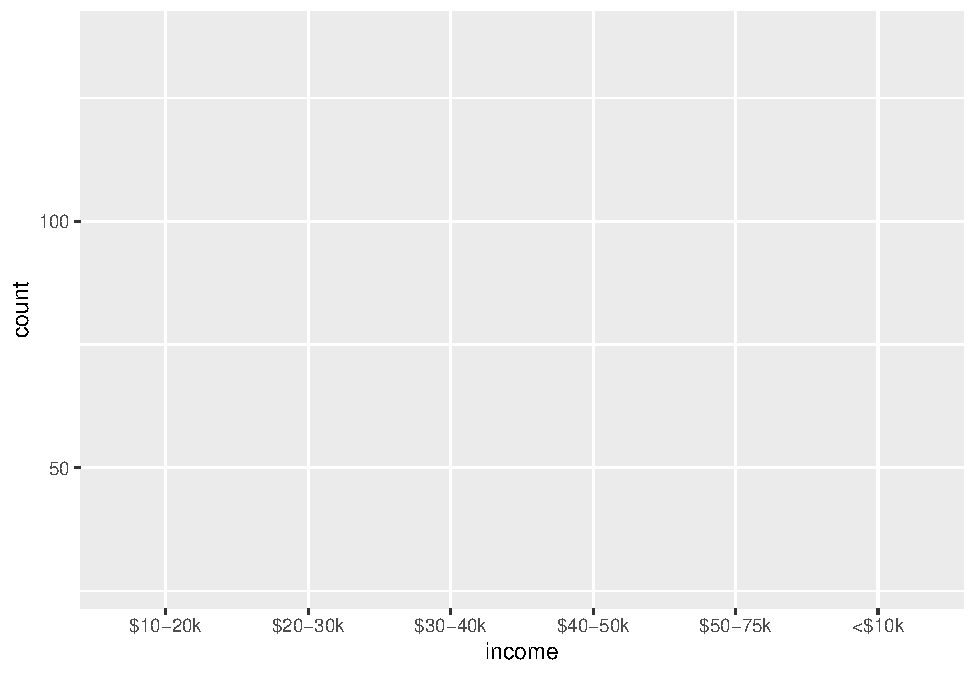
\includegraphics{bookdown-demo_files/figure-latex/unnamed-chunk-12-1.pdf}

We add an xy plot.

\begin{Shaded}
\begin{Highlighting}[]
\NormalTok{p }\OperatorTok{+}\StringTok{ }\KeywordTok{geom_point}\NormalTok{()}
\end{Highlighting}
\end{Shaded}

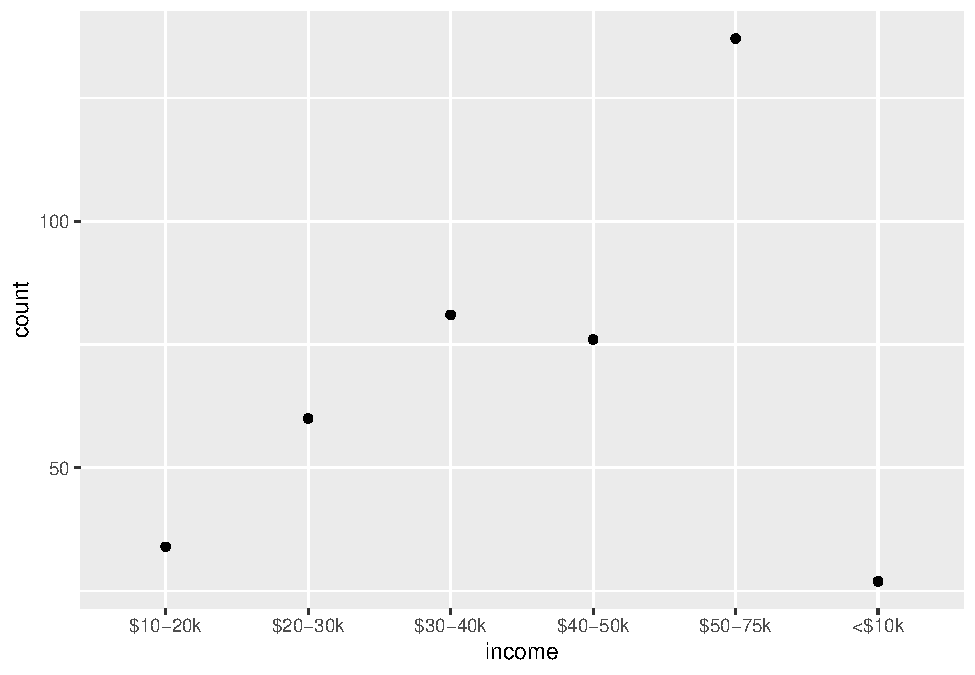
\includegraphics{bookdown-demo_files/figure-latex/unnamed-chunk-13-1.pdf}

We can also create a bar plot.

\begin{Shaded}
\begin{Highlighting}[]
\NormalTok{p }\OperatorTok{+}\StringTok{ }\KeywordTok{geom_bar}\NormalTok{(}\DataTypeTok{stat =} \StringTok{"identity"}\NormalTok{)}
\end{Highlighting}
\end{Shaded}

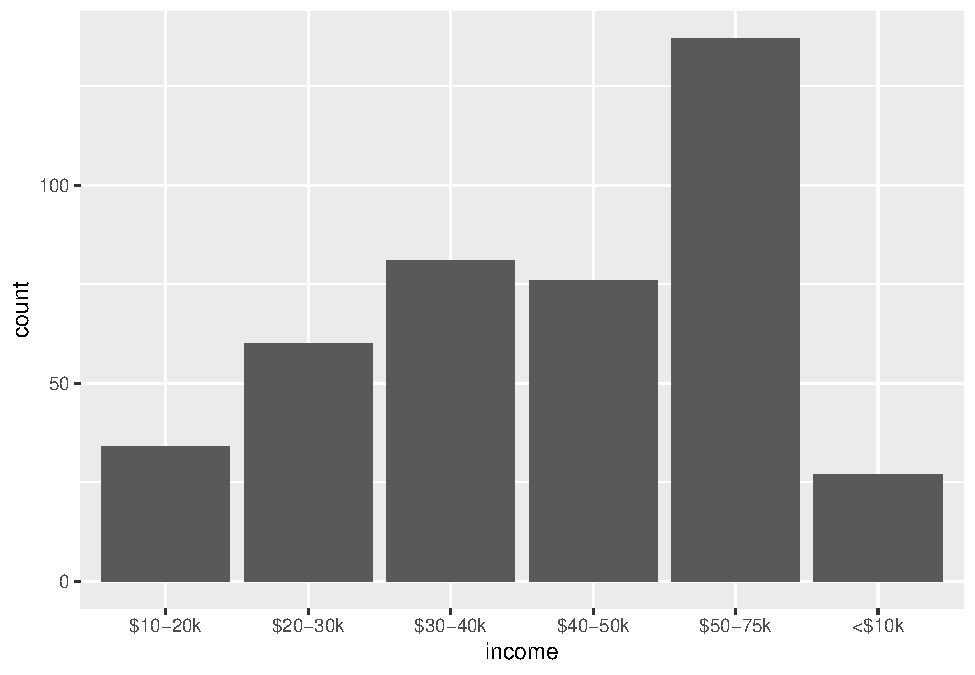
\includegraphics{bookdown-demo_files/figure-latex/unnamed-chunk-14-1.pdf}

Creating histograms is even easier. Just specify the column that you want to graph as the x column. No y is needed because a histogram is one-dimensional.

Take a x to be a random variable from a gamma distribution.

\begin{Shaded}
\begin{Highlighting}[]
\NormalTok{gamma =}\StringTok{ }\KeywordTok{tibble}\NormalTok{(}\DataTypeTok{x =} \KeywordTok{rgamma}\NormalTok{(}\DecValTok{1000}\NormalTok{, }\DataTypeTok{shape =} \DecValTok{1}\NormalTok{, }\DataTypeTok{rate =} \DecValTok{2}\NormalTok{))}
\end{Highlighting}
\end{Shaded}

\begin{Shaded}
\begin{Highlighting}[]
\NormalTok{p <-}\StringTok{ }\NormalTok{gamma }\OperatorTok\StringTok{ }\KeywordTok{ggplot}\NormalTok{(}\KeywordTok{aes}\NormalTok{(}\DataTypeTok{x =}\NormalTok{ x))}
\NormalTok{p }\OperatorTok{+}\StringTok{ }\KeywordTok{geom_histogram}\NormalTok{()}
\end{Highlighting}
\end{Shaded}

\begin{verbatim}
## `stat_bin()` using `bins = 30`. Pick better value with `binwidth`.
\end{verbatim}

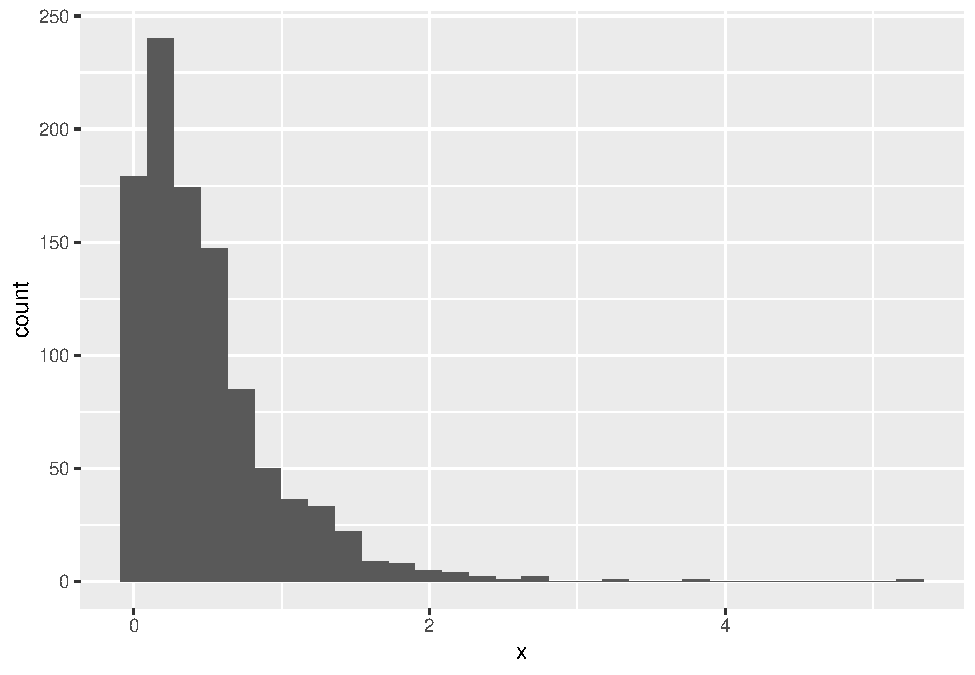
\includegraphics{bookdown-demo_files/figure-latex/unnamed-chunk-16-1.pdf}

We can graph a density instead of a histogram by using \texttt{geom\_density} instead of \texttt{geom\_hist}.

\begin{Shaded}
\begin{Highlighting}[]
\NormalTok{p }\OperatorTok{+}\StringTok{ }\KeywordTok{geom_density}\NormalTok{(}\DataTypeTok{fill =} \StringTok{"grey"}\NormalTok{)}
\end{Highlighting}
\end{Shaded}

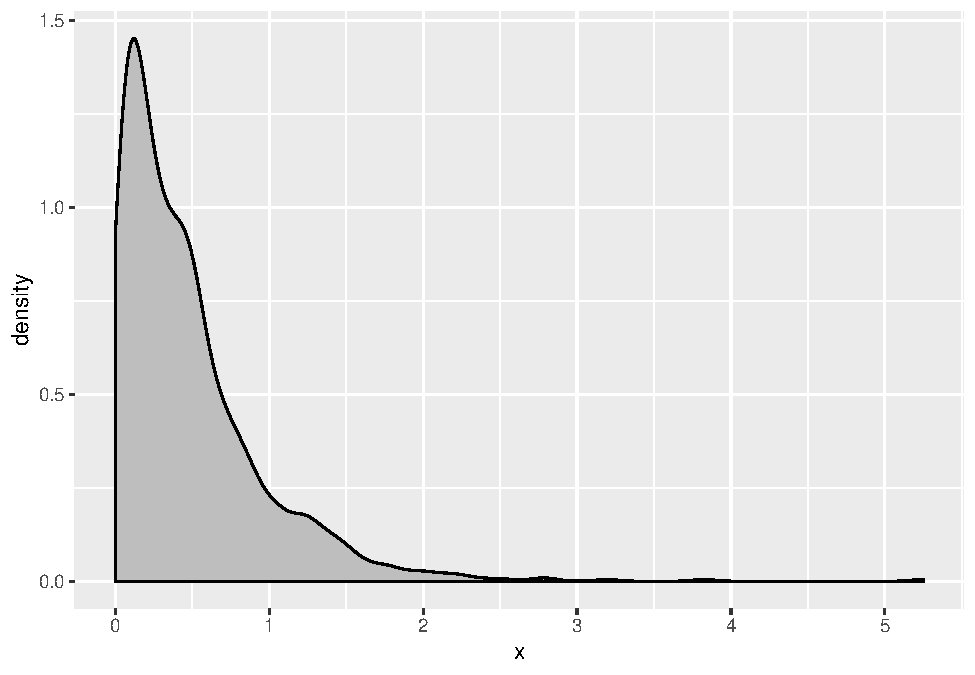
\includegraphics{bookdown-demo_files/figure-latex/unnamed-chunk-17-1.pdf}

\hypertarget{modeling}{%
\chapter{Modeling}\label{modeling}}

\hypertarget{what-is-machine-learning}{%
\section{What is machine learning}\label{what-is-machine-learning}}

All of use are already familiar with how to learn - by learning from our mistakes. By repeating what is successful and avoiding what results in failure, we ``learn'' by doing, by experience, or trial-and-error. Some methods work well for learning, but other methods do not. We all know that memorizing answers without understanding concepts is an ineffective method, and that doing many practice problems is better than doing only a few. These ideas apply to how computers learn as much as they do to how humans learn.

Take the example of preparing for an actuarial exam. We can clearly state our objective: get as many correct answers as possible!
We want to correctly predict the solution to every problem.

\[Y = \text{Problem Solution}, \hat{Y} = \text{Your Answer}\]

Said another way, we are trying to minimize the error, the percentage of incorrect problems. When \(Y = \hat{Y}\), we answer the question correctly. When \(Y \neq \hat{Y}\), we answer incorrectly.

\[\text{Exam Score} = \sum{(Y = \hat{Y})}\]

The ``data'' are the exam questions. We want to learn the patterns from the data to create a ``model'' for answering new questions.

\[X = \text{Exam Questions}\]

The ``training data'' are the practice problems. The SOA suggests 100 hours per hour of exam, which means that actuaries prepare hundreds of problems before the real exam. Often we see the same problems multiple times, and can then peak by looking at the solution. This can result in us ``overfitting'' our model if we are not careful.

The more practice problems that we do, the larger the training data set, and the better the model becomes. As we see more examples, our mental ``model'' improves. When we see new problems, ones which have not appeared in the practice exams, we often have a difficult time. Problems which we have seen before are easier, and we have more confidence in our answers.

To speed up the training time, we can ``downsample'' the data by skipping problems randomly. For example, we can only do odd-numbered problems. This insured that we still get the same proportion of each type of question while doing fewer problems.

One way to be extra-confident in our answers to to do the problem multiple ways. In modeling, using the averages of different models produces the best results.

If we use the wrong loss function our model will fail. If instead of looking at ``Correct Answers'' when practicing, we do not bother to look at the answer but instead only look at ``Number of Study Hours'', the model will not perform well on the real exam. The brain will ``learn'' to maximize study time, by taking longer time to relax and waste time, rather than aiming to get the correct answer.

X = {[}x1,x2,x3{]}
y-hat = f(X)

error = y - y\_hat

R2, RMSE, MSE, MAE, accuracy, log loss, etc

\hypertarget{a-mini-exam-example}{%
\chapter{A Mini-Exam Example}\label{a-mini-exam-example}}

The easiest way to understand this exam is to look at an example.

\hypertarget{project-statement}{%
\section{Project Statement}\label{project-statement}}

ABC Health Insurance company is building a model to predict medical claims. Using only \texttt{age} and \texttt{sex} information from the prior year, build a model to predict claims for the next year.

\hypertarget{describe-the-data-1-point}{%
\subsection{\#1 - Describe the data (1 point)}\label{describe-the-data-1-point}}

\begin{Shaded}
\begin{Highlighting}[]
\KeywordTok{library}\NormalTok{(tidyverse)}
\NormalTok{data <-}\StringTok{ }\KeywordTok{read_csv}\NormalTok{(}\StringTok{"C:/Users/sam.castillo/Desktop/R Manual Data/health_insurance.csv"}\NormalTok{) }\OperatorTok\StringTok{ }
\StringTok{  }\KeywordTok{select}\NormalTok{(age, sex, charges) }\OperatorTok\StringTok{  }\CommentTok{#put this into an r library}
\StringTok{  }\KeywordTok{rename}\NormalTok{(}\DataTypeTok{claims =}\NormalTok{ charges)}
\end{Highlighting}
\end{Shaded}

\begin{verbatim}
## Parsed with column specification:
## cols(
##   age = col_double(),
##   sex = col_character(),
##   bmi = col_double(),
##   children = col_double(),
##   smoker = col_character(),
##   region = col_character(),
##   charges = col_double()
## )
\end{verbatim}

\begin{Shaded}
\begin{Highlighting}[]
\NormalTok{data }\OperatorTok\StringTok{ }\KeywordTok{summary}\NormalTok{()}
\end{Highlighting}
\end{Shaded}

\begin{verbatim}
##       age            sex                claims     
##  Min.   :18.00   Length:1338        Min.   : 1122  
##  1st Qu.:27.00   Class :character   1st Qu.: 4740  
##  Median :39.00   Mode  :character   Median : 9382  
##  Mean   :39.21                      Mean   :13270  
##  3rd Qu.:51.00                      3rd Qu.:16640  
##  Max.   :64.00                      Max.   :63770
\end{verbatim}

\begin{Shaded}
\begin{Highlighting}[]
\NormalTok{data }\OperatorTok\StringTok{ }\KeywordTok{dim}\NormalTok{()}
\end{Highlighting}
\end{Shaded}

\begin{verbatim}
## [1] 1338    3
\end{verbatim}

\begin{quote}
The data consists of 1,338 policies with age and sex information. The objective is to predict future claims.
\end{quote}

\hypertarget{create-a-histogram-of-the-claims-and-comment-on-the-shape-1-point}{%
\subsection{\#2 - Create a histogram of the claims and comment on the shape (1 point)}\label{create-a-histogram-of-the-claims-and-comment-on-the-shape-1-point}}

The distribution of claims is strictly positive and right skewed.

\begin{Shaded}
\begin{Highlighting}[]
\NormalTok{data }\OperatorTok\StringTok{ }\KeywordTok{ggplot}\NormalTok{(}\KeywordTok{aes}\NormalTok{(claims)) }\OperatorTok{+}\StringTok{ }\KeywordTok{geom_histogram}\NormalTok{()}
\end{Highlighting}
\end{Shaded}

\begin{verbatim}
## `stat_bin()` using `bins = 30`. Pick better value with `binwidth`.
\end{verbatim}

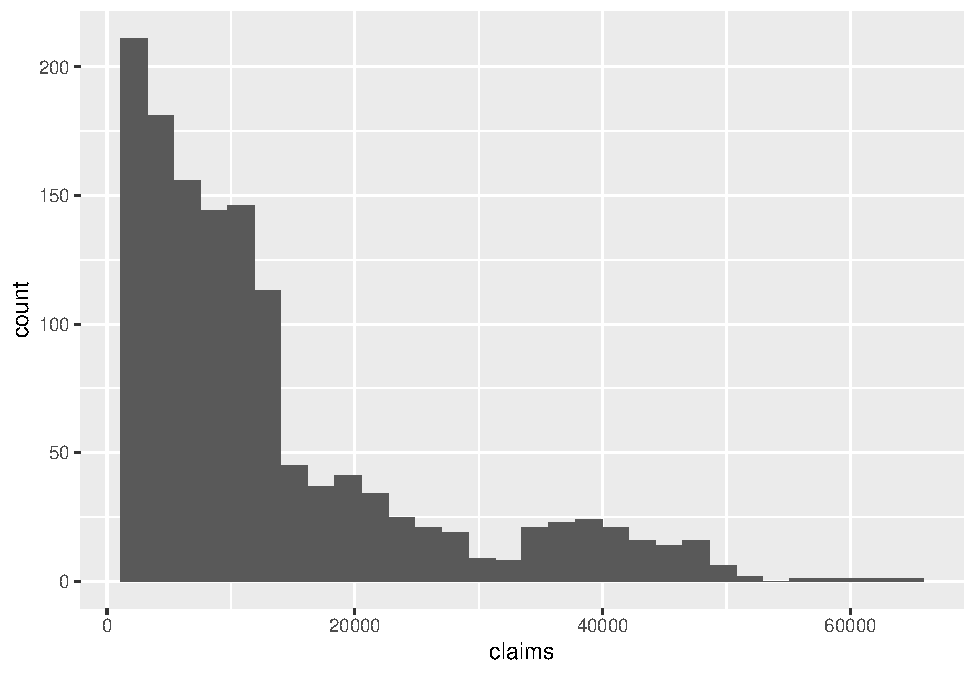
\includegraphics{bookdown-demo_files/figure-latex/unnamed-chunk-19-1.pdf}

\hypertarget{fit-a-linear-model-1-point}{%
\subsection{\#3 - Fit a linear model (1 point)}\label{fit-a-linear-model-1-point}}

\begin{Shaded}
\begin{Highlighting}[]
\NormalTok{model =}\StringTok{ }\KeywordTok{lm}\NormalTok{(claims }\OperatorTok{~}\StringTok{ }\NormalTok{age }\OperatorTok{+}\StringTok{ }\NormalTok{sex, }\DataTypeTok{data =}\NormalTok{ data)}
\end{Highlighting}
\end{Shaded}

\hypertarget{describe-the-relationship-between-age-sex-and-claim-costs-1-point}{%
\subsection{\#4 - Describe the relationship between age, sex, and claim costs (1 point)}\label{describe-the-relationship-between-age-sex-and-claim-costs-1-point}}

\begin{quote}
We fit a linear model to the claim costs using age and sex as predictor variables. The coefficient of \texttt{age} is 258, indicating that the claim costs increase by \$258 for every one-unit increase in the policyholder's age. The cofficient of 1538 on \texttt{sexmale} indicates that on average, men have \$1538 higher claims than women do.
\end{quote}

\begin{Shaded}
\begin{Highlighting}[]
\KeywordTok{coefficients}\NormalTok{(model)}
\end{Highlighting}
\end{Shaded}

\begin{verbatim}
## (Intercept)         age     sexmale 
##   2343.6249    258.8651   1538.8314
\end{verbatim}

\hypertarget{write-a-summary-of-steps-1-4-in-non-technical-language-1-point}{%
\subsection{\#5 - Write a summary of steps 1-4 in non-technical language (1 point)}\label{write-a-summary-of-steps-1-4-in-non-technical-language-1-point}}

\begin{quote}
ABC Health is interested in predicting the future claims for a group of policyholders. We began by collecting data on 1,538 policy holders which recorded their age, sex, and annual claims. We then created a histogram of the claim costs. A linear model which shows that claim costs increase as age increases, and are higher for men on average.
\end{quote}

\bibliography{book.bib,packages.bib}


\end{document}
